\documentclass[12pt]{article}
%\usepackage{caption}
\usepackage{setspace,graphicx,epstopdf,amsmath,amsfonts,amssymb,amsthm}
\usepackage{marginnote,datetime,enumitem,subfigure,rotating,fancyvrb}
\usepackage{hyperref,float}
\usepackage[longnamesfirst]{natbib}
\usepackage{mathtools}
\usepackage{caption}
\usepackage{float}
\usepackage{lscape}
\usepackage{graphicx}
\usepackage{flafter} 
\usepackage{tabularx} 
\usepackage{booktabs}
\usepackage{changepage}
\usepackage{setspace}
\usepackage{placeins}
\usepackage{threeparttable}
\usepackage{ragged2e}
\usepackage[export]{adjustbox}
\newcolumntype{Y}{>{\raggedleft\arraybackslash}X}% raggedleft column X
\usdate
\usepackage[a4paper,bindingoffset=0.2in,%
            left=1.1in,right=0.85in,top=1in,bottom=1in,%
            footskip=.25in]{geometry}


% SCRIPTS:
% used SP19_rm_27 to create all the tables with monthly returns

% Number paragraphs and subparagraphs and include them in TOC
\setcounter{tocdepth}{2}

% JF-specific includes:

\usepackage{indentfirst} % Indent first sentence of a new section.
\usepackage{endnotes}    % Use endnotes instead of footnotes


\begin{document}

\setlist{noitemsep}  % Reduce space between list items (itemize, enumerate, etc.)
\onehalfspacing      % Use 1.5 spacing
% Use endnotes instead of footnotes - redefine \footnote command
\renewcommand{\footnote}{\endnote}  % Endnotes instead of footnotes

\author{Mykola Pinchuk\thanks{\rm Simon Business School, University of Rochester. Email: Mykola.Pinchuk@ur.rochester.edu. \newline I would like to thank Alan Moreira, Shuaiyu Chen, Xuyanda Qi and David Swanson for helpful comments.}}

\title{\Large \bf Cross-Industry Dispersion and Expected Retruns}

\date{05 September 2019}             % Final submission before Oct. 15

% Create title page with no page number

\maketitle
\thispagestyle{empty}

\bigskip

%\normalsize

\centerline{\bf ABSTRACT}

\small
\begin{onehalfspace}  % Double-space the abstract and don't indent it
  \noindent This paper examines cross-industry dispersion (CID), defined as a mean absolute deviation of returns of 49 industry portfolios. I find that expected stock returns are related cross-sectionally to the sensitivities of returns to innovations in CID. Annualized returns of the stocks with high sensitivity to CID are 8.4\% lower than the returns of the stocks with low sensitivity. This return spread is not explained by common factors, since abnormal returns with respect to the best factor model exceed 6\%. The results can arise due to across-industry labor income risk.
\end{onehalfspace}
\normalsize
\medskip


\clearpage
%\doublespacing
\setstretch{1.6}


\section{Introduction} \label{sec:Model}
Economy is a dynamic system with permanently evolving structure. As some industries are born, the other industries are losing their importance. A few people in 1970s could have predicted that within 20 years IT sector would capture the largest share of the stock market. There is no reason to expect a constant rate of this structural transformation. Naturally, accelerated structural tranformation increases aggregate economic uncertainty and labor market risk for workers in underperforming industries. This paper explores asset pricing implications of such structural uncertainty.
\paragraph{}
I document a novel evidence that stock exposures to cross-industry dispersion (CID) can predict cross section of expected returns. CID is defined as mean absolute deviation of the returns of 49 industry portfolios. The paper finds that the firms with large return sensitivity to CID deliver smaller returns than the stocks with low sensitivity to CID. This finding suggests that in equilibrium there exists an extra demand for stocks, positively comoving with CID, implying low expected returns of these stocks. Long-short portfolio, formed on the sensitivity to CID, delivers monthly return of 70 bps with abnormal returns of 50 bps.
\paragraph{}
This evidence is consistent with several sources of risk, possibly related to CID. Periods of highly nonhomogeneous performance of different industries (high CID) are likely to be the periods of increased economic uncertainty. Times of large wedge in the performance of winning and losing industries can proxy for the periods of rapid economic transformation, when some industries become more important, while the others lose relevance. During these periods investors are likely to have less understanding of the economic environment, reflecting growing uncertainty. Moreover, economy is more vulnerable to shocks within such uncertain times. Alternatively, high CID may indicate temporary decrease in output and efficiency as resources are reallocated across sectors (Lilien 1982). Since risk-averse agents lose utility when uncertainty rises, they create hedging demand for the stocks, whose returns positively comove with CID.
\paragraph{}
Labor income risk is another possible channel, explaining relevance of CID to asset pricing. By construction, high CID means that some industries severely underperform the market, while the others enjoy exceptionally high returns. This pattern is likely to raise a concern that losing industry is under the threat of dying. Naturally, this is a period of a negative shock to expected lifetime labor income of the employees in underperforming industries. The fact that there are both outperforming and underperforming industries with returns sufficiently far from the market return implies even larger labor income risk that the one during the recession. Within the recession, the common wisdom is that most of lost jobs will be recovered at some point in the future, while disappearance of some industry means loss of the jobs forever. 
\paragraph{}
While many occupations are demanded across different industries, they are usually low skill occupations, less relevant to asset pricing. Losing high-wage job constitutes larger negative shock to lifetime income. Moreover, high-paid workers are likely to have larger savings and produce larger effect in financial market. High-skill jobs (e.g., aerospace engineer) are usually confined to a few industries, implying very low across-industry labor mobility. Thus, I expect that CID captures asset pricing effect of Cross-sectional Dispersion (CSD), consistent with labor income risk. According to labor income risk explanation, stocks with negative covariance with CID are more risky, since they tend to fall when the risk of losing high skill industry-immobile jobs is large.
\paragraph{}
This paper draws upon the theoretical contribution of Duffie and Constantinides (1996) to motivate CIV as a state variable. Duffie and Constantinides show that in the model with heterogeneous agents, subject to uninsurable labor income shocks, cross-sectional variance of agnets` consumption growth becomes a state variable. As discussed above, severe underperformance of their industry suggests a negative shock to expected consumption growth of employees.
\paragraph{}
This study contributes to several domains of literature. Different measures of market volatility have traditionally been used as a proxy for economic and financial uncertainty. Ang et al (2006) empirically show that exposure of stocks to VIX is priced in cross-section of expected stock returns. Kelly et al (2016) report that stocks with larger sensitivity to common idiosyncratic volatility (CIV) earn lower expected returns. They argue that CIV proxies for idiosyncratic risk faced by households and suggest labor income risk as a main channel.
\paragraph{}
This article builds upon a body of labor literature. Lilien (1982) reports that sectoral shifts and performance dispersion result in unemployment shocks, caused by migration of employees between firms and sectors. Loungani, Rush and Tave (1990) construct stock market dispersion index and document that it predicts unemployment. Brainard and Cutler (1993) use similar measure to assess the contribution of sectoral reallocation to unemployment. They find that sectoral reallocation accounts for large share of unemployment fluctuations at long horizons. Multiple studies (Blundell et al 2008, ) document that households can not completely insure their consumption from persistent shocks to their labor income. These findings highlight the importance of labor income risk for asset pricing.
\paragraph{}
The idea of cross-sectional dispersion of some economic variable as a measure of uncertainty has been extensively used with accounting variables instead of returns. Bloom (2009) documents strong correlation between time-series measures of market volatility, cross-sectional variation of firms` pretax profit growth and returns and dispersion across macroeconomic forecasts. He argues that all of these variables proxy for financial and macroeconomic uncertainty. Sadka (2012) finds that higher earnings dispersion is associated with higher expected returns, suggesting that earnings dispersion is a state variable, relevant for asset pricing.
\paragraph{}
This paper is closely related to the literature on cross-sectional dispersion (CSD), defined as a standard (mean absolute) deviation of the cross section of stock returns. Bekaert and Harvey (1997, 2000) use CSD as a measure of development and maturity of the stock market. Stivers (2003, 2006, 2010) finds that CSD can predict idiosyncratic volatility as well as returns of value and momentum premia. Maio (2013, 2016) reports that cross-sectional standard deviation of returns of the portfolios, sorted on size and book-to-market can predict market returns. The closest paper to this one is Verousis and Voukelatos (2018). It finds that the stocks with high sensitivity to CSD offer lower returns in the 1996-2012 sample. Due to more idiosyncratic nature of CSD, the authors explain the findings by idiosyncratic risk without elaborating on or providing evidence for this explanation.
\paragraph{}
This paper uses 1963-2018 sample and shows that sensitivities to CID predict lower expected returns. I argue that this predictability stems from return dispersion across industries, proxying for labor income risk due to sectoral changes. The results suggest that only across-industry component of CSD (i.e., CID) is priced. Long-short portfolio, formed on CID, controlling for CSD, delivers 32 bps (t-statistic=2.46) monthly returns, while long-short portfolio, formed on CSD, controlling for CID, produces -3 bps returns. 
% there was the paper Jiang(2010), which seems totally retarded to me. the guy found 26% annualized quintile spread using beta from regression of returns on levels and explained it with the risk story with the wrong sign. do not want to cite it %.








\section{Data and Dispersion Measures} \label{sec:Model}
\subsection{Sample}
\subsection{Construction of Dispersion Measures}


\section{Asset Pricing Results} \label{sec:Model}
This section documents and discusses the main results of the paper. 
\subsection{Estimation of $\beta_{CID}$}
\begin{center}
[Insert Table 2 here] 
\end{center}
\subsection{Portfolios, formed on $\beta_{CID}$}
\subsection{Cross-sectional Results}
\subsection{Performance of different Dispersion Measures}


\section{Economic Channel: Labor Income Risk} \label{sec:Model}
\subsection{Economic Mechanism and Hypotheses}
\subsection{Results}


\section{Further results} \label{sec:Model}
\subsection{Robustness to different industry definitions}
\subsection{Robustness to other uncertainty measures}
\subsection{Results at lower frequency}
\subsection{Economic and financial forecasting power of CIV}

\newpage

\section{Conclusion} \label{sec:Model}


\newpage
\section{References:}
\begin{enumerate}


    \item {Fama, Eugene F., and James D. MacBeth. "Risk, return, and equilibrium: Empirical tests." Journal of political economy 81, no. 3 (1973): 607-636.}
    \item {Fama, E. F., \& French, K. R. (2015). A five-factor asset pricing model. Journal of Financial Economics, 116(1), 1–22. }
    \item {Harvey, Campbell R., Yan Liu, and Heqing Zhu. "… and the cross-section of expected returns." The Review of Financial Studies 29, no. 1 (2016): 5-68.}
    \item {Hong, Harrison, Walter Torous, and Rossen Valkanov. "Do industries lead stock markets?." Journal of Financial Economics 83, no. 2 (2007): 367-396.}
    \item {Hou, Kewei, and Tobias J. Moskowitz. "Market frictions, price delay, and the cross-section of expected returns." The Review of Financial Studies 18, no. 3 (2005): 981-1020.}
    \item {Hou, Kewei, Chen Xue, and Lu Zhang. "Digesting anomalies: An investment approach." The Review of Financial Studies 28, no. 3 (2015): 650-705.}
     \item {Jensen, Michael C., Fischer Black, and Myron S. Scholes. "The capital asset pricing model: Some empirical tests." (1972).}
    \item {Menzly, Lior, and Oguzhan Ozbas. "Market segmentation and cross‐predictability of returns." The Journal of Finance 65, no. 4 (2010): 1555-1580.}


\end{enumerate}

\newpage


\newgeometry{left=2.5cm, right=0.75cm, top=1.75cm, bottom=1.5cm}
\section*{Appendix}

\begin{figure*}
\textbf{Figure 1: Dispersion Measures}
\vskip 6 pt
\begin{flushleft}
{The plot describes time series of cross-sectional dispersion (CSD), cross-industry dispersion (CID) and within-industry dispersion (WID). All the measures are calculated as mean absolute deviation of the returns at daily frequency. Industries are defined according to Fama-French 49 industry classification. The paper uses value-weighted industry returns to calculate CID.}
\end{flushleft}
\centering
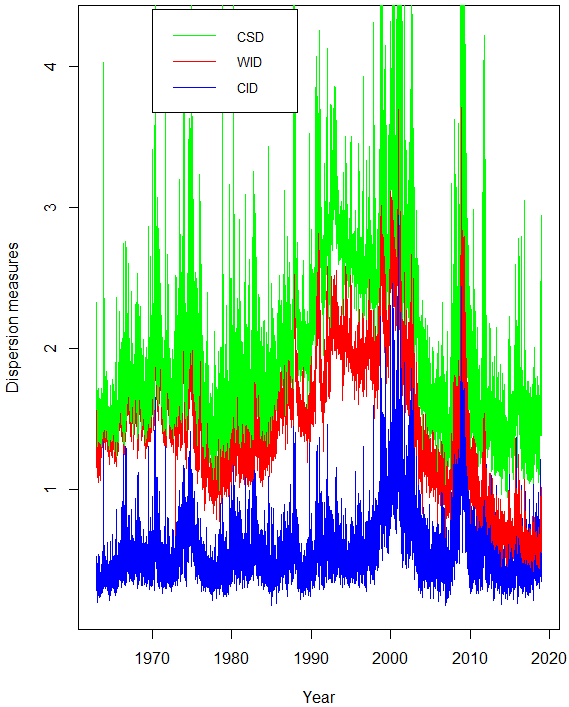
\includegraphics[width=1\textwidth]{fig1.png}
\end{figure*}


\begin{figure*}
\textbf{Figure 2: Postranking $\beta_{CID}$}
\vskip 12 pt
\begin{flushleft}
{The plot describes the relationship between postranking and preranking $\beta_{CID}$ of decile portfolios, sorted on $\beta_{CID}$.}
\end{flushleft}
\centering
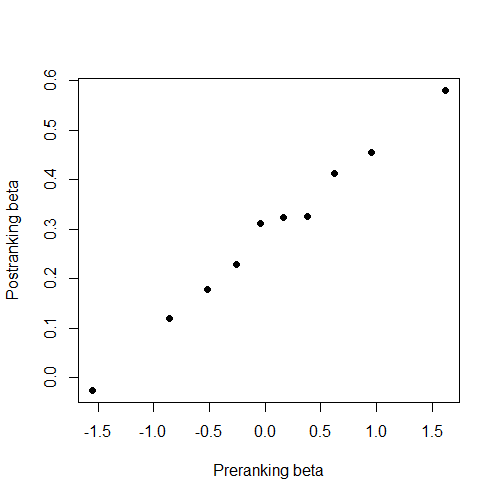
\includegraphics[width=1\textwidth]{Figure2.png}
\end{figure*}


\begin{figure*}
\textbf{Figure 3: Performance of \$1 (log scale)}
\vskip 12 pt
\begin{flushleft}
{The plot describes growth of the investment of \$1 in one of the three portfolios. L/S5 (L/S10) corresponds to long-short portfolio, defined as a difference in returns of extreme quintile (decile) portfolios. Mkt is the value-weighted return of all CRSP stocks(vwretd).}
\end{flushleft}
\centering
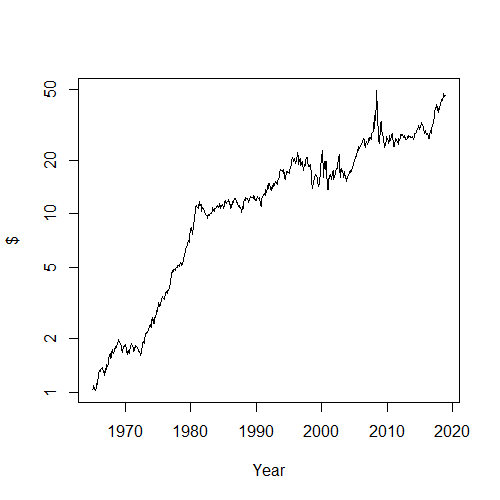
\includegraphics[width=1\textwidth]{Figure3.png}
\end{figure*}


\begin{figure*}
\textbf{Figure 4: Returns of decile L/S portfolio using different Fama-French industry partitions}
\vskip 12 pt
\begin{flushleft}
{The plot describes monthly returns and abnormal returns of decile L/S portfolios, formed on $\beta_{CID}$. I use Fama-French industry definitions with different coarseness: 49, 30, 17, 10 and 5 industries to compute CID. Abnormal returns are calculated with respect to Fama-French 5 factor model, including Momentum and Short-term Reversal factors.}
\end{flushleft}
\centering
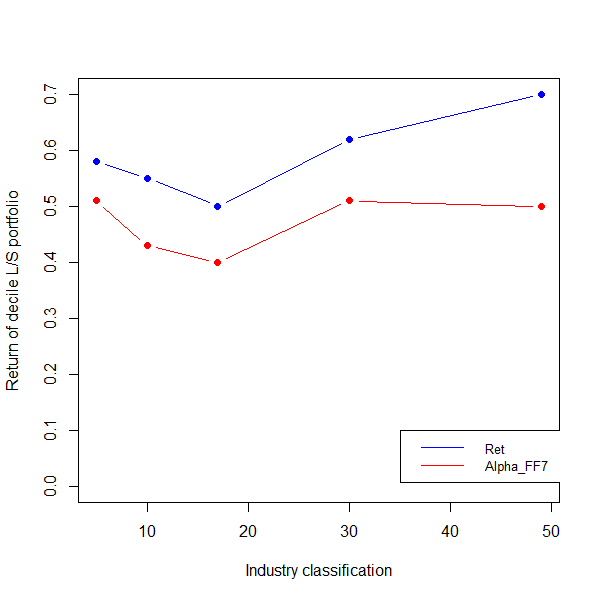
\includegraphics[width=1\textwidth]{alphas_inds.png}
\end{figure*}


\clearpage


% Table created by stargazer v.5.2.2 by Marek Hlavac, Harvard University. E-mail: hlavac at fas.harvard.edu
% Date and time: Tue, Sep 03, 2019 - 1:38:31 PM
\begin{table}[!htbp] \centering 
  \caption{Correlations of changes in CID with changes of other variables} 
  \label{} 
    \begin{flushleft}
    {\medskip\small
 The table reports correlations between changes in CID and changes in other variables at monthly frequency. VIX is implied volatility, available starting from 1990. FU and MU are financial and macroeconomic uncertainty from Sydney Ludvigson website. VOL is the volatility of monthly value-weighted market index over recent 24 months. CIV is common idosyncratic volatility (Kelly et al., 2016). }
    \medskip
    \end{flushleft}
\begin{tabular}{@{\extracolsep{5pt}} ccccccc} 
\\[-1.8ex]\hline 
\hline \\[-1.8ex] 
 & VIX & FU & MU & VOL & CIV & CID \\ 
\hline \\[-1.8ex] 
VIX & $1$ & $0.40$ & $0.36$ & $0.34$ & $0.50$ & $0.12$ \\ 
FU & $0.40$ & $1$ & $0.44$ & $0.30$ & $0.39$ & $0.26$ \\ 
MU & $0.36$ & $0.44$ & $1$ & $0.11$ & $0.24$ & $0.09$ \\ 
VOL & $0.34$ & $0.30$ & $0.11$ & $1$ & $0.27$ & $0.29$ \\ 
CIV & $0.50$ & $0.39$ & $0.24$ & $0.27$ & $1$ & $0.30$ \\ 
CID & $0.12$ & $0.26$ & $0.09$ & $0.29$ & $0.30$ & $1$ \\ 
\hline \\[-1.8ex] 
\end{tabular} 
\end{table}



% Table created by stargazer v.5.2.2 by Marek Hlavac, Harvard University. E-mail: hlavac at fas.harvard.edu
% Date and time: Tue, Sep 03, 2019 - 1:39:07 PM
\begin{table}[!htbp] \centering 
  \caption{Characteristics of decile $\beta_{CID}$-sorted vw portfolios} 
  \label{} 
      \begin{flushleft}
    {\medskip\small
 The table reports mean values of characteristics of decile portfolios, sorted on $\beta_{CID}$. Size is log of market equity in the previous month. bm is log of Book-to-Market. op is operating profitability. BAspr is average bid-ask spread as a percentage of average price over the previous month. }
    \medskip
    \end{flushleft}
\begin{tabular}{@{\extracolsep{0pt}} lccccccccccc} 
\\[-1.8ex]\hline 
\hline \\[-1.8ex] 
 & D1 & D2 & D3 & D4 & D5 & D6 & D7 & D8 & D9 & D10 & LS \\ 
\hline \\[-1.8ex] 
RET & $1.17$ & $0.88$ & $0.86$ & $0.71$ & $0.63$ & $0.65$ & $0.65$ & $0.60$ & $0.52$ & $0.47$ & $$-$0.70$ \\ 
RET\_tstat & $4.80$ & $4.38$ & $4.56$ & $3.97$ & $3.73$ & $3.87$ & $3.69$ & $3.48$ & $2.79$ & $2.12$ & $$-$3.87$ \\ 
preranking beta & $$-$1.55$ & $$-$0.86$ & $$-$0.51$ & $$-$0.26$ & $$-$0.05$ & $0.16$ & $0.38$ & $0.62$ & $0.96$ & $1.62$ & $3.16$ \\ 
postranking beta & $$-$0.03$ & $0.12$ & $0.18$ & $0.23$ & $0.31$ & $0.32$ & $0.33$ & $0.41$ & $0.46$ & $0.58$ & $0.62$ \\ 
size & $7.11$ & $7.71$ & $8.13$ & $8.37$ & $8.60$ & $8.81$ & $8.96$ & $9.16$ & $9.15$ & $8.85$ & $1.74$ \\ 
bm & $6.05$ & $6.12$ & $6.13$ & $6.14$ & $6.14$ & $6.11$ & $6.11$ & $6.07$ & $6.01$ & $5.97$ & $$-$0.08$ \\ 
op & $0.15$ & $0.16$ & $0.17$ & $0.17$ & $0.17$ & $0.17$ & $0.17$ & $0.18$ & $0.18$ & $0.17$ & $0.02$ \\ 
inv & $0.29$ & $0.23$ & $0.18$ & $0.16$ & $0.14$ & $0.13$ & $0.13$ & $0.14$ & $0.14$ & $0.17$ & $$-$0.12$ \\ 
beta & $1.07$ & $0.96$ & $0.91$ & $0.88$ & $0.88$ & $0.89$ & $0.92$ & $0.98$ & $1.08$ & $1.31$ & $0.23$ \\ 
BAspr & $0.39$ & $0.32$ & $0.26$ & $0.24$ & $0.23$ & $0.21$ & $0.20$ & $0.19$ & $0.18$ & $0.18$ & $$-$0.21$ \\ 
mom122 & $0.24$ & $0.18$ & $0.15$ & $0.14$ & $0.12$ & $0.12$ & $0.11$ & $0.11$ & $0.11$ & $0.14$ & $$-$0.10$ \\ 
vol1m & $2.47$ & $2.02$ & $1.82$ & $1.72$ & $1.66$ & $1.61$ & $1.60$ & $1.63$ & $1.74$ & $2.03$ & $$-$0.44$ \\ 
vol12m & $2.63$ & $2.12$ & $1.90$ & $1.79$ & $1.72$ & $1.68$ & $1.67$ & $1.71$ & $1.83$ & $2.19$ & $$-$0.43$ \\ 
\hline \\[-1.8ex] 
\end{tabular} 
\end{table}




% Table created by stargazer v.5.2.2 by Marek Hlavac, Harvard University. E-mail: hlavac at fas.harvard.edu
% Date and time: Tue, Sep 03, 2019 - 2:31:38 PM
\begin{table}[!htbp] \centering 
  \caption{Returns of decile $\beta_{CID}$-sorted portfolios} 
  \label{} 
\begin{tabular}{@{\extracolsep{-5pt}} cccccccccccc} 
\\[-1.8ex]\hline 
\hline \\[-1.8ex] 
 & D1 & D2 & D3 & D4 & D5 & D6 & D7 & D8 & D9 & D10 & LS \\ 
\hline \\[-1.8ex] 
Mean ew & 2.50 & 1.79$^{***}$ & 1.58$^{***}$ & 1.41$^{***}$ & 1.36$^{***}$ & 1.32$^{***}$ & 1.29$^{***}$ & 1.26$^{***}$ & 1.29$^{***}$ & 1.61$^{***}$ & -0.89$^{***}$ \\ 
T-stat ew & 9.65 & 8.70 & 8.15 & 7.73 & 7.48 & 7.26 & 6.84 & 6.52 & 6.34 & 6.45 & -5.72 \\ 
Mean vw & 1.17 & 0.88$^{***}$ & 0.86$^{***}$ & 0.71$^{***}$ & 0.63$^{***}$ & 0.65$^{***}$ & 0.65$^{***}$ & 0.60$^{***}$ & 0.52$^{***}$ & 0.47$^{**}$ & -0.70$^{***}$ \\ 
T-stat vw & 4.80 & 4.38 & 4.56 & 3.97 & 3.73 & 3.87 & 3.69 & 3.48 & 2.79 & 2.12 & -3.87 \\ 
\hline \\[-1.8ex] 
\end{tabular} 
\end{table}



% Table created by stargazer v.5.2.2 by Marek Hlavac, Harvard University. E-mail: hlavac at fas.harvard.edu
% Date and time: Tue, Sep 03, 2019 - 1:44:52 PM
\begin{table}[!htbp] \centering 
  \caption{Abnormal returns of decile $\beta_{CID}$-sorted vw portfolios} 
  \label{} 
\begin{tabular}{@{\extracolsep{0pt}} ccccccc} 
\\[-1.8ex]\hline 
\hline \\[-1.8ex] 
Statistic & Ret & $\alpha_{CAPM}$ & $\alpha_{FF3}$ & $\alpha_{Carhart}$ & $\alpha_{FF5}$ & $\alpha_{FF5+UMD+STR}$ \\ 
\hline \\[-1.8ex] 
LS & -0.70$^{***}$ & -0.67$^{***}$ & -0.75$^{***}$ & -0.55$^{***}$ & -0.80$^{***}$ & -0.50$^{***}$ \\ 
 & [ -3.87] & [ -3.68] & [ -4.44] & [ -3.24] & [ -4.59] & [ -2.90] \\ 
\hline \\[-1.8ex] 
\end{tabular} 
\end{table}



% Table created by stargazer v.5.2.2 by Marek Hlavac, Harvard University. E-mail: hlavac at fas.harvard.edu
% Date and time: Tue, Sep 03, 2019 - 1:45:59 PM
\begin{table}[!htbp] \centering 
  \caption{Factor loadings of decile $\beta_{CID}$-sorted vw portfolios} 
  \label{} 
\begin{tabular}{@{\extracolsep{0pt}} ccccccccccc} 
\\[-1.8ex]\hline 
\hline \\[-1.8ex] 
Decile & Ret & Alpha & EMKT & HML & SMB & RMW & CMA & Mom & STR & adjR2 \\ 
\hline \\[-1.8ex] 
1 & 1.17 & 0.57 & 1.03 & -0.07 & 0.42 & -0.23 & -0.34 & 0.16 & 0.12 & 0.83 \\ 
 & [ 4.80] & [ 5.24] & [ 38.82] & [ -1.37] & [ 11.75] & [ -4.61] & [ -4.57] & [ 6.39] & [ 3.41] &  \\ 
2 & 0.88 & 0.22 & 0.97 & 0.05 & 0.23 & 0.07 & -0.15 & 0.12 & 0.10 & 0.84 \\ 
 & [ 4.38] & [ 2.46] & [ 45.09] & [ 1.18] & [ 7.84] & [ 1.63] & [ -2.43] & [ 5.67] & [ 3.48] &  \\ 
3 & 0.86 & 0.28 & 0.95 & 0.03 & 0.13 & -0.02 & -0.10 & 0.12 & 0.04 & 0.84 \\ 
 & [ 4.56] & [ 3.40] & [ 47.65] & [ 0.66] & [ 4.98] & [ -0.45] & [ -1.75] & [ 6.48] & [ 1.60] &  \\ 
4 & 0.71 & 0.07 & 0.96 & 0.03 & 0.08 & 0.14 & 0.05 & 0.08 & 0.07 & 0.86 \\ 
 & [ 3.97] & [ 0.92] & [ 54.98] & [ 1.00] & [ 3.56] & [ 4.13] & [ 1.03] & [ 4.67] & [ 2.99] &  \\ 
5 & 0.63 & 0.00 & 0.94 & 0.04 & 0.08 & 0.14 & 0.17 & 0.05 & 0.01 & 0.88 \\ 
 & [ 3.73] & [ -0.02] & [ 60.62] & [ 1.43] & [ 3.60] & [ 4.91] & [ 3.97] & [ 3.37] & [ 0.64] &  \\ 
6 & 0.65 & 0.07 & 0.92 & 0.02 & -0.01 & 0.13 & 0.10 & 0.02 & 0.06 & 0.88 \\ 
 & [ 3.87] & [ 1.20] & [ 60.34] & [ 0.70] & [ -0.27] & [ 4.62] & [ 2.33] & [ 1.38] & [ 3.11] &  \\ 
7 & 0.65 & 0.08 & 0.98 & 0.03 & -0.04 & 0.11 & 0.13 & -0.02 & 0.05 & 0.90 \\ 
 & [ 3.69] & [ 1.36] & [ 67.63] & [ 1.10] & [ -1.81] & [ 3.84] & [ 3.25] & [ -1.65] & [ 2.72] &  \\ 
8 & 0.60 & 0.03 & 1.01 & 0.12 & -0.08 & 0.18 & 0.12 & -0.04 & 0.00 & 0.91 \\ 
 & [ 3.48] & [ 0.47] & [ 74.54] & [ 4.69] & [ -4.30] & [ 7.16] & [ 3.14] & [ -2.98] & [ -0.24] &  \\ 
9 & 0.52 & 0.04 & 1.03 & 0.07 & -0.10 & 0.05 & 0.08 & -0.09 & -0.03 & 0.88 \\ 
 & [ 2.79] & [ 0.60] & [ 60.97] & [ 2.13] & [ -4.17] & [ 1.59] & [ 1.59] & [ -5.27] & [ -1.37] &  \\ 
10 & 0.47 & 0.07 & 1.16 & 0.14 & -0.04 & -0.12 & -0.11 & -0.13 & -0.13 & 0.83 \\ 
 & [ 2.12] & [ 0.71] & [ 47.98] & [ 3.07] & [ -1.15] & [ -2.71] & [ -1.64] & [ -5.54] & [ -3.96] &  \\ 
LS & -0.70 & -0.50 & 0.13 & 0.21 & -0.46 & 0.11 & 0.23 & -0.29 & -0.25 & 0.23 \\ 
 & [ -3.87] & [ -2.90] & [ 3.04] & [ 2.62] & [ -8.05] & [ 1.35] & [ 1.94] & [ -7.20] & [ -4.41] &  \\ 
\hline \\[-1.8ex] 
\end{tabular} 
\end{table} 



% Table created by stargazer v.5.2.2 by Marek Hlavac, Harvard University. E-mail: hlavac at fas.harvard.edu
% Date and time: Tue, Sep 03, 2019 - 1:47:00 PM
\begin{table}[!htbp] \centering 
  \caption{Abnormal returns of 2x3 doublesorted portfolios on size and $\beta_{CID}$} 
  \label{} 
\begin{tabular}{@{\extracolsep{5pt}} ccccccc} 
\\[-1.8ex]\hline 
\hline \\[-1.8ex] 
Statistic & Ret & $\alpha_{CAPM}$ & $\alpha_{FF3}$ & $\alpha_{Carhart}$ & $\alpha_{FF5}$ & $\alpha_{FF5+UMD+STR}$ \\ 
\hline \\[-1.8ex] 
L/S Size & 0.74$^{***}$ & 0.67$^{***}$ & 0.51$^{***}$ & 0.56$^{***}$ & 0.47$^{***}$ & 0.52$^{***}$ \\ 
T-stat & [ 7.38] & [ 6.84] & [ 12.35] & [ 13.92] & [ 11.30] & [ 12.66] \\ 
L/S CID & 0.22$^{**}$ & 0.23$^{**}$ & 0.28$^{***}$ & 0.15 & 0.31$^{***}$ & 0.16 \\ 
T-stat & [ 2.24] & [ 2.40] & [ 2.91] & [ 1.59] & [ 3.13] & [ 1.61] \\ 
\hline \\[-1.8ex] 
\end{tabular} 
\end{table}



% Table created by stargazer v.5.2.2 by Marek Hlavac, Harvard University. E-mail: hlavac at fas.harvard.edu
% Date and time: Wed, Sep 04, 2019 - 10:02:03 AM
\begin{table}[!htbp] \centering 
  \caption{Fama-MacBeth regression} 
  \label{} 
\begin{tabular}{@{\extracolsep{0pt}}lccccccc} 
\\[-1.8ex]\hline 
\hline \\[-1.8ex] 
 & \multicolumn{7}{c}{\textit{Dependent variable: Return}} \\ 
\cline{2-8} 
\\[-1.8ex] & (1) & (2) & (3) & (4) & (5) & (6) & (7)\\ 
\hline \\[-1.8ex] 
 $\beta_{CID}$ & $-$0.30$^{***}$ & $-$0.31$^{***}$ & $-$0.09$^{**}$ & $-$0.10$^{**}$ & $-$0.09$^{**}$ & $-$0.09$^{***}$ & $-$0.09$^{***}$ \\ 
  & [ $-$4.64] & [ $-$6.50] & [ $-$2.45] & [ $-$2.53] & [ $-$2.39] & [ $-$2.60] & [ $-$2.60] \\ 
  & & & & & & & \\ 
 $\beta_{MKT}$ &  & 0.31 & 0.69$^{***}$ & 0.71$^{***}$ & 0.64$^{***}$ & 0.72$^{***}$ & 0.62$^{***}$ \\ 
  &  & [ 1.54] & [ 3.11] & [ 3.35] & [ 3.17] & [ 3.59] & [ 3.25] \\ 
  & & & & & & & \\ 
 size &  &  & $-$0.63$^{***}$ & $-$0.62$^{***}$ & $-$0.62$^{***}$ & $-$0.62$^{***}$ & $-$0.58$^{***}$ \\ 
  &  &  & [ $-$14.36] & [ $-$13.63] & [ $-$13.98] & [ $-$14.24] & [ $-$14.57] \\ 
  & & & & & & & \\ 
 logbm &  &  &  & 0.04 & 0.05 & $-$0.02 & 0.004 \\ 
  &  &  &  & [ 0.77] & [ 0.90] & [ $-$0.28] & [ 0.07] \\ 
  & & & & & & & \\ 
 mom122 &  &  &  &  & 0.04 & 0.01 & 0.02 \\ 
  &  &  &  &  & [ 0.22] & [ 0.04] & [ 0.13] \\ 
  & & & & & & & \\ 
 inv &  &  &  &  &  & $-$1.23$^{***}$ & $-$1.25$^{***}$ \\ 
  &  &  &  &  &  & [ $-$8.34] & [ $-$8.51] \\ 
  & & & & & & & \\ 
 MAX &  &  &  &  &  &  & 0.02$^{***}$ \\ 
  &  &  &  &  &  &  & [ 3.21] \\ 
  & & & & & & & \\ 
 Constant & 1.49$^{***}$ & 1.21$^{***}$ & 4.58$^{***}$ & 4.51$^{***}$ & 4.49$^{***}$ & 4.56$^{***}$ & 4.26$^{***}$ \\ 
  & [ 7.61] & [ 9.42] & [ 16.03] & [ 15.68] & [ 15.93] & [ 16.38] & [ 16.41] \\ 
  & & & & & & & \\ 
\hline \\[-1.8ex] 
Observations & 1,254,089 & 1,254,089 & 1,254,089 & 1,254,089 & 1,253,020 & 1,226,228 & 1,226,045 \\ 
Adjusted R$^{2}$ & 0.01 & 0.04 & 0.05 & 0.06 & 0.07 & 0.07 & 0.07 \\ 
\hline 
\hline \\[-1.8ex] 
\textit{Note:}  & \multicolumn{7}{r}{$^{*}$p$<$0.1; $^{**}$p$<$0.05; $^{***}$p$<$0.01} \\ 
\end{tabular} 
\end{table}


\clearpage


% Table created by stargazer v.5.2.2 by Marek Hlavac, Harvard University. E-mail: hlavac at fas.harvard.edu
% Date and time: Tue, Sep 03, 2019 - 1:47:48 PM
\begin{table}[!htbp] \centering 
  \caption{Abnormal returns of 5x5 doublesorted portfolios on within-industry dispersion $\beta_{WID}$ and $\beta_{CID}$} 
  \label{} 
\begin{tabular}{@{\extracolsep{5pt}} ccccccc} 
\\[-1.8ex]\hline 
\hline \\[-1.8ex] 
Statistic & Ret & $\alpha_{CAPM}$ & $\alpha_{FF3}$ & $\alpha_{Carhart}$ & $\alpha_{FF5}$ & $\alpha_{FF5+UMD+STR}$ \\ 
\hline \\[-1.8ex] 
L/S WID & 0.13 & 0.22 & 0.09 & -0.03 & -0.16 & -0.19 \\ 
T-stat & [ 0.89] & [ 1.46] & [ 0.61] & [ -0.19] & [ -1.08] & [ -1.27] \\ 
L/S CID & 0.38$^{***}$ & 0.34$^{**}$ & 0.44$^{***}$ & 0.38$^{***}$ & 0.59$^{***}$ & 0.43$^{***}$ \\ 
T-stat & [ 2.75] & [ 2.33] & [ 3.16] & [ 2.72] & [ 4.27] & [ 3.06] \\ 
\hline \\[-1.8ex] 
\end{tabular} 
\end{table}



% Table created by stargazer v.5.2.2 by Marek Hlavac, Harvard University. E-mail: hlavac at fas.harvard.edu
% Date and time: Tue, Sep 03, 2019 - 1:48:32 PM
\begin{table}[!htbp] \centering 
  \caption{Abnormal returns of 5x5 doublesorted portfolios on cross-sectional dispersion $\beta_{CSD}$ and $\beta_{CID}$} 
  \label{} 
\begin{tabular}{@{\extracolsep{5pt}} ccccccc} 
\\[-1.8ex]\hline 
\hline \\[-1.8ex] 
Statistic & Ret & $\alpha_{CAPM}$ & $\alpha_{FF3}$ & $\alpha_{Carhart}$ & $\alpha_{FF5}$ & $\alpha_{FF5+UMD+STR}$ \\  
\hline \\[-1.8ex] 
L/S CSD & -0.03 & 0.07 & -0.03 & -0.15 & -0.21 & -0.32$^{**}$ \\ 
T-stat & [ -0.20] & [ 0.49] & [ -0.24] & [ -1.06] & [ -1.52] & [ -2.24] \\ 
L/S CID & 0.32$^{**}$ & 0.28$^{**}$ & 0.30$^{**}$ & 0.26$^{**}$ & 0.43$^{***}$ & 0.31$^{**}$ \\ 
T-stat & [ 2.46] & [ 2.06] & [ 2.36] & [ 2.00] & [ 3.31] & [ 2.38] \\ 
\hline \\[-1.8ex] 
\end{tabular} 
\end{table}

\begin{table}[!htbp] \centering 
  \caption{Abnormal returns of 5x5 doublesorted portfolios on cross-sectional dispersion $\beta_{CSD}$ and other variables} 
  \label{} 
\begin{tabularx}{\linewidth}{p{2cm}p{1.5cm}p{1.5cm}p{1.5cm}p{1.5cm}p{1.5cm}p{1.5cm}}
    \toprule
    \multicolumn{7}{l}{\textbf{Panel A: VIX vs CID}} \\
    \midrule  
\\[-1.8ex]\hline 
\hline \\[-1.8ex] 
Statistic & Ret & $\alpha_{CAPM}$ & $\alpha_{FF3}$ & $\alpha_{Carhart}$ & $\alpha_{FF5}$ & $\alpha_{FF5+UMD+STR}$ \\ 
\hline \\[-1.8ex] 
L/S VIX & 0.25 & -0.13 & -0.09 & 0.05 & 0.19 & 0.28 \\ 
T-stat & [ 1.08] & [ -0.68] & [ -0.49] & [ 0.30] & [ 1.10] & [ 1.61] \\ 
L/S CID & 0.24 & 0.24 & 0.38$^{**}$ & 0.22 & 0.30 & 0.15 \\ 
T-stat & [ 1.20] & [ 1.19] & [ 2.12] & [ 1.24] & [ 1.64] & [ 0.87] \\ 
\hline \\[-1.8ex] 
\end{tabularx} 

\begin{tabularx}{\linewidth}{p{2cm}p{1.5cm}p{1.5cm}p{1.5cm}p{1.5cm}p{1.5cm}p{1.5cm}}
    \toprule
    \multicolumn{7}{l}{\textbf{Panel B: CIV vs CID}} \\
    \midrule  
\\[-1.8ex]\hline 
\hline \\[-1.8ex] 
Statistic & Ret & $\alpha_{CAPM}$ & $\alpha_{FF3}$ & $\alpha_{Carhart}$ & $\alpha_{FF5}$ & $\alpha_{FF5+UMD+STR}$ \\ 
\hline \\[-1.8ex] 
L/S CIV & 0.33$^{***}$ & 0.27$^{**}$ & 0.16 & 0.21$^{*}$ & 0.08 & 0.13 \\ 
T-stat & [ 2.75] & [ 2.25] & [ 1.41] & [ 1.76] & [ 0.66] & [ 1.04] \\ 
L/S CID & 0.37$^{***}$ & 0.39$^{***}$ & 0.42$^{***}$ & 0.26$^{**}$ & 0.44$^{***}$ & 0.23$^{**}$ \\ 
T-stat & [ 3.06] & [ 3.22] & [ 3.64] & [ 2.27] & [ 3.70] & [ 1.99] \\ 
\hline \\[-1.8ex] 
\end{tabularx} 


\begin{tabularx}{\linewidth}{p{2cm}p{1.5cm}p{1.5cm}p{1.5cm}p{1.5cm}p{1.5cm}p{1.5cm}}
    \toprule
    \multicolumn{7}{l}{\textbf{Panel C: Macroeconomic uncertainty (Ludvigson15) vs CID}} \\
    \midrule  
\\[-1.8ex]\hline 
\hline \\[-1.8ex] 
Statistic & Ret & $\alpha_{CAPM}$ & $\alpha_{FF3}$ & $\alpha_{Carhart}$ & $\alpha_{FF5}$ & $\alpha_{FF5+UMD+STR}$ \\ 
\hline \\[-1.8ex] 
L/S MU & 0.05 & -0.07 & -0.03 & 0.08 & 0.19 & 0.19 \\ 
T-stat & [ 0.33] & [ -0.50] & [ -0.20] & [ 0.56] & [ 1.43] & [ 1.44] \\ 
L/S CID & 0.49$^{***}$ & 0.49$^{***}$ & 0.53$^{***}$ & 0.35$^{***}$ & 0.54$^{***}$ & 0.32$^{**}$ \\ 
T-stat & [ 3.76] & [ 3.74] & [ 4.19] & [ 2.82] & [ 4.20] & [ 2.55] \\ 
\hline \\[-1.8ex] 
\end{tabularx} 

\begin{tabularx}{\linewidth}{p{2cm}p{1.5cm}p{1.5cm}p{1.5cm}p{1.5cm}p{1.5cm}p{1.5cm}}
    \toprule
    \multicolumn{7}{l}{\textbf{Panel D: Financial uncertainty (Ludvigson15) vs CID}} \\
    \midrule 
\\[-1.8ex]\hline 
\hline \\[-1.8ex] 
Statistic & Ret & $\alpha_{CAPM}$ & $\alpha_{FF3}$ & $\alpha_{Carhart}$ & $\alpha_{FF5}$ & $\alpha_{FF5+UMD+STR}$ \\ 
\hline \\[-1.8ex] 
L/S FU & 0.25$^{*}$ & 0.15 & 0.01 & -0.04 & -0.10 & -0.07 \\ 
T-stat & [ 1.85] & [ 1.14] & [ 0.07] & [ -0.29] & [ -0.79] & [ -0.53] \\ 
L/S CID & 0.39$^{***}$ & 0.40$^{***}$ & 0.44$^{***}$ & 0.31$^{***}$ & 0.45$^{***}$ & 0.28$^{**}$ \\ 
T-stat & [ 3.25] & [ 3.27] & [ 3.75] & [ 2.69] & [ 3.70] & [ 2.33] \\ 
\hline \\[-1.8ex] 
\end{tabularx} 

\begin{tabularx}{\linewidth}{p{2cm}p{1.5cm}p{1.5cm}p{1.5cm}p{1.5cm}p{1.5cm}p{1.5cm}}
    \toprule
    \multicolumn{7}{l}{\textbf{Panel E: Market volatility vs CID}} \\
    \midrule 
\\[-1.8ex]\hline 
\hline \\[-1.8ex] 
Statistic & Ret & $\alpha_{CAPM}$ & $\alpha_{FF3}$ & $\alpha_{Carhart}$ & $\alpha_{FF5}$ & $\alpha_{FF5+UMD+STR}$ \\ 
\hline \\[-1.8ex] 
L/S VOL & 0.30$^{**}$ & 0.18 & 0.25$^{**}$ & 0.29$^{**}$ & 0.49$^{***}$ & 0.47$^{***}$ \\ 
T-stat & [ 2.22] & [ 1.36] & [ 1.96] & [ 2.18] & [ 3.85] & [ 3.64] \\ 
L/S CID & 0.40$^{***}$ & 0.42$^{***}$ & 0.45$^{***}$ & 0.32$^{***}$ & 0.48$^{***}$ & 0.30$^{**}$ \\ 
T-stat & [ 3.31] & [ 3.45] & [ 3.84] & [ 2.72] & [ 4.00] & [ 2.48] \\ 
\hline \\[-1.8ex] 
\end{tabularx} 
\end{table} 










\end{document}

